\documentclass[11pt, oneside]{article} 
\usepackage{geometry}
\geometry{letterpaper} 
\usepackage{graphicx}
	
\usepackage{amssymb}
\usepackage{amsmath}
\usepackage{parskip}
\usepackage{color}
\usepackage{hyperref}

\graphicspath{{/Users/telliott/Dropbox/Github-Math/quickgeo/figures/}{/Users/telliott/Dropbox/Github-Math/figures/}}
% \begin{center} \includegraphics [scale=0.4] {gauss3.png} \end{center}

\title{Ceva}
\date{}

\begin{document}
\maketitle
\Large

%[my-super-duper-separator]

When we draw a line from each vertex in a triangle to the side opposite, those lines have different names depending on how we pick the end-point.  Some possibilities are:

$\circ$ \ to form the perpendicular (altitude)

$\circ$ \ to bisect the side (median)

$\circ$ \ to bisect the angle where we start

These three lines always seem to cross at the same point.  Here, we look at the conditions under which this happens.  Start with the altitude.

In $\triangle ABC$ draw two of the altitudes, from $A$ and $B$.
\begin{center} 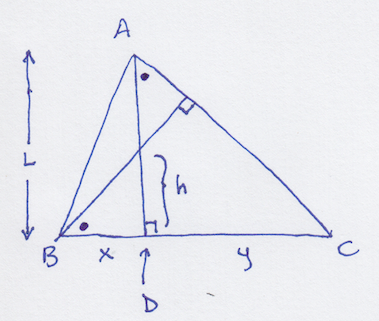
\includegraphics [scale=0.6] {K1.png} \end{center}
The altitude from the vertex $A$ meets the base in a right angle at $D$.  This altitude divides the base into lengths $x$ and $y$.  

Now draw a second altitude from vertex $B$ to the side opposite.  

What is the height $h$ above the base where the two lines cross?

The two small triangles formed by the junction of the altitudes are similar.  They share vertical angles and both are right triangles, so the angles marked with a dot are equal.

But the large $\triangle ACD$ is also a right triangle and contains the same dotted angle so it is similar to the first two.

The ratio of the base lengths for the lower small triangle is $h/x$, and that for $\triangle ACD$ is $y/L$.  ($h$ and $y$ go on top because they are opposite the dotted angle).

As similar triangles
\[ \frac{h}{x} = \frac{y}{L} \]
\[ h = \frac{xy}{L} \]

The formula is really interesting.  It is symmetrical in $x$ and $y$ and it does not contain any term related to the length of side $AB$.  

Therefore, if we draw the third altitude to side $AB$ and then calculate the height for it above the intersection with $AD$, we will get the same answer.
\begin{center} 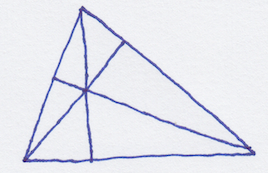
\includegraphics [scale=0.6] {K1a.png} \end{center}

And this means that the three altitudes cross at a single point.  Newton published this proof about 1680.  This is a proof of existence for the orthocenter, and of concurrence, for the altitudes.

\begin{center} \includegraphics [scale=0.5] {/Users/telliott/Dropbox/Github-Math/figures/newton3.png} \end{center}

One other idea about the orthocenter.  We can draw a circle around any triangle.  If we do that, and apply the theorem on chords that cross in a circle, we can draw an extension of any altitude to the circle beneath it.  Call that extension $g$.  The crossed chords theorems says that the product of the chord segments are equal:
\[ xy = gL \]
Rearranging what we had above gives
\[ xy = hL \]
So $g = h$.  The extension of the altitude to meet the circumcircle is equal to the height of the orthocenter above the side to which the altitude has been drawn.

\begin{center} 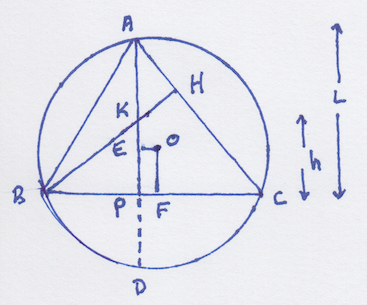
\includegraphics [scale=0.6] {K9.png} \end{center}
\[ PD = PK \]

\subsection*{median}

Next, we look at a median.  The line from vertex $B$ is drawn to bisect the opposite side.
\begin{center} 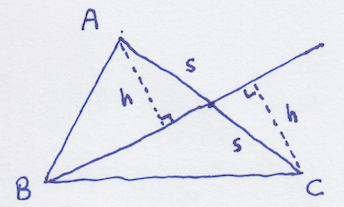
\includegraphics [scale=0.6] {K2.png} \end{center}

The altitudes from $A$ and $C$ to the median are drawn.  This forms two small triangles that are congruent, since $s = s$ and we have two (three) angles equal.  Therefore, the altitudes are the same length.

We conclude that the median divides the original triangle into two smaller triangles with the shared base and equal altitudes, so they have the same area.

Now we think about the general case.
\begin{center} 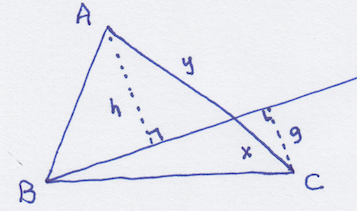
\includegraphics [scale=0.6] {K3.png} \end{center}

Here, $x \ne y$.  But we still have two similar triangles formed by the altitudes $g$ and $h$  By similar triangles the altitudes are in the same ratio as the bases:
\[ \frac{g}{h} = \frac{x}{y} \]

Again the base is shared.  Therefore the areas of the two triangles formed by the solid line have their areas in the same ratio as the bases $x:y$.  

Here is a diagram for another proof for the same conclusion.

\begin{center} 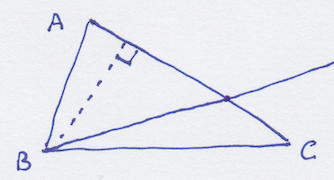
\includegraphics [scale=0.6] {K4.png} \end{center}

\subsection*{Menelaus' theorem}

We come now to a theorem by Menelaus.  We are headed for Ceva's theorem.  I have heard that theorem is too hard to be taught in high school, but that's because they generally use a complicated proof.  Menelaus' theorem makes it easy, and Menelaus is itself easy, so we're going to do them both.

There are multiple possibilities for a proof of Menelaus' theorem, we will look at one Einstein valued for its symmetry.

In a triangle, draw the \emph{traversal}, the solid line in the middle, that meets the extended base on the right.
\begin{center} 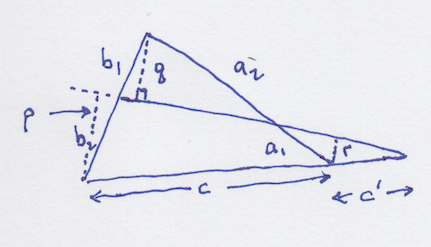
\includegraphics [scale=0.6] {K5.png} \end{center}

The sides are divided into lengths $a_1$ and $a_2$, and $b_1$ and $b_2$.  The extended base is labeled with a prime to emphasize the extension.  Three altitudes are drawn as well.

From similar triangles we can write
\[ \frac{r}{p} = \frac{c'}{c + c'}, \ \ \ \ \ \ \frac{p}{q} = \frac{b_2}{b_1}, \ \ \ \ \ \ \frac{q}{r} = \frac{a_2}{a_1} \]

Since the left-hand sides, multiplied together are equal to $1$, so is the product of the right-hand sides.
\[ 1 = \frac{c'}{c + c'} \cdot \frac{b_2}{b_1} \cdot \frac{a_2}{a_1} \]

which we can rewrite as
\[ 1 = \frac{a_1}{a_2} \cdot \frac{b_1}{b_2} \cdot \frac{c + c'}{c'} \]

$\square$

\begin{center} 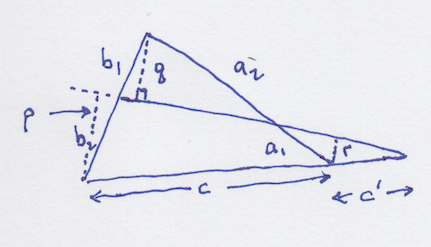
\includegraphics [scale=0.6] {K5.png} \end{center}

Going around the circle from whichever vertex is convenient, we take the lengths in the order that we first encounter them, remembering that $c$ and $c'$ are not like the other two.

\subsection*{Ceva's theorem}

Finally, we come to Ceva's theorem.
\begin{center} 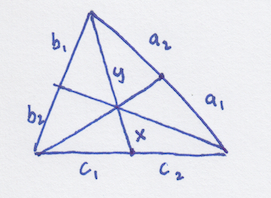
\includegraphics [scale=0.6] {K6.png} \end{center}

Draw three lines crossing at any point $P$ in the interior of the triangle.

Let us apply Menelaus' theorem to the two half triangles formed by the line drawn from the apex to the base.  For the left we have that
\[ 1 = \frac{x}{y} \cdot \frac{b_1}{b_2} \cdot \frac{c_1 + c_2}{c_2} \]

The other one is taken in the clockwise direction (or form the mirror image):
\[ 1 = \frac{x}{y} \cdot \frac{a_2}{a_1} \cdot \frac{c_1 + c_2}{c_1} \]

Equating the two expressions and canceling $x/y$ and $c_1 + c_2$ we obtain
\[ \frac{b_1}{b_2} \cdot \frac{1}{c_2} = \frac{a_2}{a_1} \cdot \frac{1}{c_1} \]

which can be rearranged to give:
\[ \frac{a_1}{a_2} \cdot \frac{b_1}{b_2} \cdot \frac{c_1}{c_2} = 1 \]

If the lines meet at the center, then the proportions of the parts of the sides multiply to give $1$.

\begin{center} 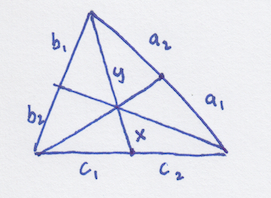
\includegraphics [scale=0.6] {K6.png} \end{center}

The converse theorem is also true.  Concurrence of lines follows from the fact that the product of proportions is equal to $1$.  We will skip the proof for this part, but it's relatively easy to construct a proof by contradiction.

$\square$

\subsection*{placement of the centroid}
Did you notice?  We had
\[ 1 = \frac{x}{y} \cdot \frac{b_1}{b_2} \cdot \frac{c_1 + c_2}{c_2} \]
For the case of the centroid, the middle term is $1$ and the right-hand term is $2$ so
\[ 1 = \frac{x}{y} \cdot 2 \]
\[ y = 2x \]
The centroid is one-third of the distance up from the base.

\subsection*{back to the orthocenter}

Here is a second proof of existence for the orthocenter, using Ceva's theorem directly.
\begin{center} 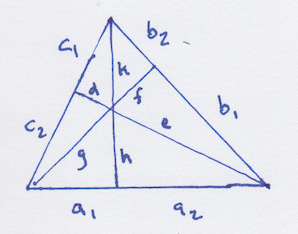
\includegraphics [scale=0.6] {K7.png} \end{center}

For each vertex, find the two right triangles that contain the entire angle.  These triangles are similar, so we can form the same ratios.  Start at the top and work clockwise:
\[ \frac{c_1}{b} = \frac{b_2}{c}, \ \ \ \ \ \ \frac{b_1}{a} = \frac{a_2}{b},  \ \ \ \ \ \  \frac{a_1}{c} = \frac{c_2}{a} \]

Notice the symmetry!
Rearranging 
\[ \frac{c_1}{b_2} = \frac{b}{c},  \ \ \ \ \ \  \frac{b_1}{a_2} = \frac{a}{b},  \ \ \ \ \ \  \frac{a_1}{c_2} = \frac{c}{a} \]
The product of the three fractions on the right-hand side is $1$, which is equal to the product of the three fractions from the left-hand side:
\[ \frac{c_1}{b_2} \cdot \frac{b_1}{a_2} \cdot \frac{a_1}{c_2} = 1 \]

$\square$

\subsection*{Euler line}

One final thought about concurrence.  There cannot be any general ratio that describes the placement of the orthocenter, where altitudes cross.  The reason is that in a right triangle, that ratio is zero because they cross at the right angle.

Let's look a little closer at an isosceles right triangle.  If you recall, we showed that the median drawn to the hypotenuse is itself a radius of the circumcircle.  So the half-way point of the hypotenuse is the circumcenter.
\begin{center} 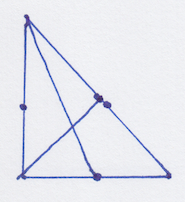
\includegraphics [scale=0.6] {K8.png} \end{center}

If we draw a line from the orthocenter, at the right angle, to the circumcenter, this \emph{is} a median of the triangle.  So the centroid, where the medians cross, lies on a line between the circumcenter and the orthocenter.

It is not difficult to show that the centroid's distance from the orthocenter is twice its distance from the median, but we will leave that to you.

Another special case is the equilateral triangle, where the altitude and the median are the same line for each vertex, or the isosceles triangles, where they are the same line for one vertex, and both go through the circumcenter.

Euler showed that both of these results hold for all triangles.   The centroid, where the medians cross, lies on a line between the circumcenter and the orthocenter.  The distance from the centroid to the orthocenter is twice the distance to the circumcenter.

We'll save that as something for the future.


\end{document}